\documentclass{beamer}

\usetheme[secheader]{Boadilla}
\usecolortheme{seahorse}
\usepackage[spanish]{babel} 		% {Con estos dos anda
\usepackage[utf8]{inputenc} 		% todo lo que es tildes y ñ}
\usepackage{verbatim}
\usepackage{alltt}
\renewcommand{\ttdefault}{txtt}

\title{HYPNOS: Understanding and Treating Sleep Conflicts in Smartphones}
\author{Martín Carreiro - Pablo Rago - Juan Manuel Tastzian}
\date{21 de Mayo de 2014}
\institute[2014]{Facultad de Ciencias Exactas y Naturales}

\begin{document}

\frame{\titlepage}

\section[Outline]{}
\frame{\tableofcontents}

\section{Introduction}

\subsection{Contexto}
\frame {
	\frametitle{Contexto}
	\begin{itemize}
		\item<1->Es la primera vez en la historia de la computación en donde la energía es un problema 
		\item<2->Mismo las notebooks, están pensadas para estar mayormente conectadas
		\item<3->Y los teléfonos tienen que durar el día entero...
		\item<4->Se introduce el Modelo de Manejo de Energía
	\end{itemize}
}

\subsection{Modelo de Manejo de Energía}
\frame {
	\frametitle{Modelo de Manejo de Energía}
    \only<1>{
	\begin{block}{Desde el CPU}
      \begin{itemize}
		\item Después de un período de inactividad, el teléfono ingresa en un estado de suspensión
		\item Esto incluye el SOC: CPU, ROM,  micro-controladores de varios dispositivos como el GPS, gráficos, video y audio
		\item La RAM ingresa en un estado de actualización
		\item El CPU intentará acceder a dicho estado cada 20ms, a menos que alguien lo interrumpa (veremos quien puede)
		\item En este estado el CPU consume casi-cero energía.
	\end{itemize}
   \end{block}	
   }
   \only<2>{
   \begin{block}{Desde el desarrollador}
      \begin{itemize}
		\item<1->Los desarrolladores tienen que manejar el estado de cada uno de los dispositivos que utiliza (GPS, WiFi, etc)
		\item<2->El manejo de energía se convierte en una preocupación primaria
		\item<2->Además de todos los bugs de la app, se tienen que manejar los Energy Bugs
		\item<2->Dolor de cabeza
	\end{itemize}
   \end{block}
   }
}

\section{Mecanismos de manejo de energía}

\frame {
	\frametitle{Mecanismos de manejo de energía}
	\begin{itemize}
	    \item Wakelocks
	    \item Suspend Notifiers
	    \item Hardware wakeups
	\end{itemize}
}

\subsection{Wakelocks}
\frame {
\frametitle{Wakelocks}
    \begin{block}{Wakelocks}
        \begin{itemize}
            \item Mecanismo de alto nivel para prevenir la suspensión del SOC. 
            \item Tienen una API mediante la cual se pueden obtener y liberar. 
            \item Opcionalmente cuando un wakelock se obtiene se puede especificar un timeout para que después de ese plazo se libere automáticamente. 
            \item Para usarlos tienen q ser inicializados lo cual los registra en el wakelock manager del kernel
        \end{itemize}    
    \end{block}
}

\subsection{Suspend notifiers}
\frame {
    \frametitle{Suspend Notifiers}
    \begin{block}{Suspend Notifiers}
        \begin{itemize}
        \item Mecanismo de bajo nivel que permite proseguir o abortar la suspensión del SOC
        \item SOC notifica a los registrados que se quiere suspender
        \item Si nadie devuelve error, se suspende el SOC
        \item Si alguien devuelve error, el proceso de suspensión es abortado
        \item Antes que esto corrobora que no haya wakelocks tomados
        \end{itemize}
    \end{block}   
}

\subsection{Hardqare wakeups}
\frame{
    \frametitle{Hardware Wakeups}
    \begin{block}{Hardware Wakeups}
        \begin{itemize}
        \item A diferencia de los anteriores, no impiden que duerma, si no que despierta al SOC cuando lo necesita.
        \item Por ejemplo el Real Time Clock (RTC). Este es esencial para soportar servicios que deben ejecutarse a intervalos fijos de tiempo. Su API permite especificar un timer con un callback. 
        \item Otros dispositivos con este poder: Wifi, wake-on-lan, llamada entrante
        \item Estos son los únicos que pueden!
        \end{itemize}
    \end{block}

}

\section{Un Tipo de Energy Bug: Sleep Conflict}
\subsection{Definición}
\frame {
	\frametitle{Un Tipo de Energy Bug: Sleep Conflict}
	Los \textit{sleep conflicts} pasan cuando un dispositivo en un estado de alto consumo de energía es incapaz de hacer la transición de vuelta al estado de energía básico porque el CPU esta dormido y el controlador del dispositivo no puede progresar en su ejecución para hacer la transición.
	\\
	Tres Factores que dan lugar a \textit{sleep conflicts}: 
	\begin{itemize}
		\item Un dispostivo puede estar en uno de varios estados de energia independientemente del estado de energia del SOC
		\item El driver del dispositivo controla las transiciones de estados de energia
		\item El SO usa una politica agresiva de suspension del sistema.
	\end{itemize}	
}
\subsection{Ejemplo}
\frame{
	\frametitle{Ejemplo}
	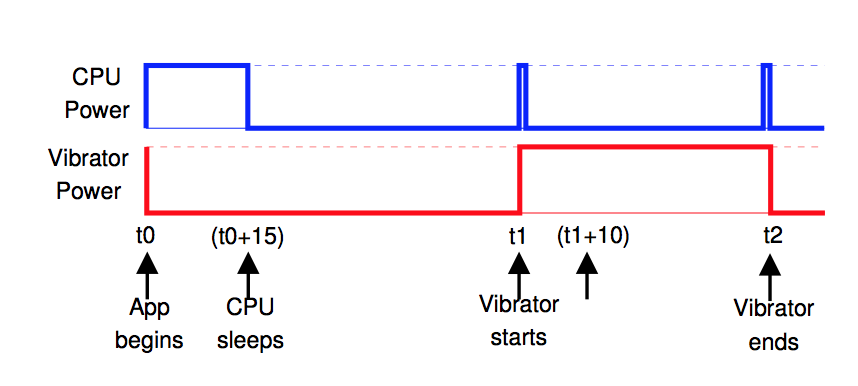
\includegraphics{vibrador.png}
}


\frame{
    \frametitle{Evitando sleep conflicts con suspend notifiers}
    \begin{itemize}
    \item Hacer que pare el dispostivo y luego permitir a la CPU suspenderse
    \item Abortar el proceso de suspensión
    \item Registrar un timer RTC que se dispare cuando el dispositivo vaya a tener que ejecutar el código que lo apaga 
    \end{itemize}
}

\subsection{Clasificación}
\frame{
    \frametitle{Clasificación de los sleep conflicts}
    \begin{itemize}
    \item Esperando a que termine la utilización activa
    \item Esperando por una transición mediante un timeout
    \item Esperando por una transición por input del programa
    \item Esperando por una transición mediante un evento externo
    \end{itemize}
}

\section{HYPNOS}

\frame{
    \frametitle{HYPNOS}
    \begin{block}{¿Qué es?}
    Es un programa que en tiempo de ejecución permite evitar bugs de sleep conflict en drivers de dispositivos. Funciona haciendo el checkeo en forma online mientras las aplicaciones se ejecutan normalmente, y ademas permite testear la aplicación en busca de sleep conflicts antes de ser deployada.
    \end{block}
}

\frame{
    \frametitle{HYPNOS}
    \begin{block}{Funcionamiento}
    El enfoque tomado para tratar los sleep conlicts es intentar evitarlos en primer lugar. Esto se logra checkeando las condiciones que podrían llevar a un sleep conflict a cada pedido de suspención del sistema. Para esto no se necesita conocer el código fuente de los drivers de los dispositivos siempre y cuando se cuente con una forma de monitorear las transiciones de energía y se tenga acceso a los modelos de FSM de cada dispositivo. Para generar los modelos de FSM de los dispositivos de un smartphone dado se realizan procesos de ingeniería inversa offline.
    \end{block}
}

\frame{
    \frametitle{HYPNOS}
    \begin{block}{Arquitectura}
    El sistema monitorea las transiciones de energía interceptando las interacciónes con el bus de los drivers y checkeando por posibles condiciones de sleep conflict justo antes de que el sistema se suspenda para ejecutar las acciones preventivas acordemente.
    \end{block}
}

\frame{
    \frametitle{HYPNOS}
    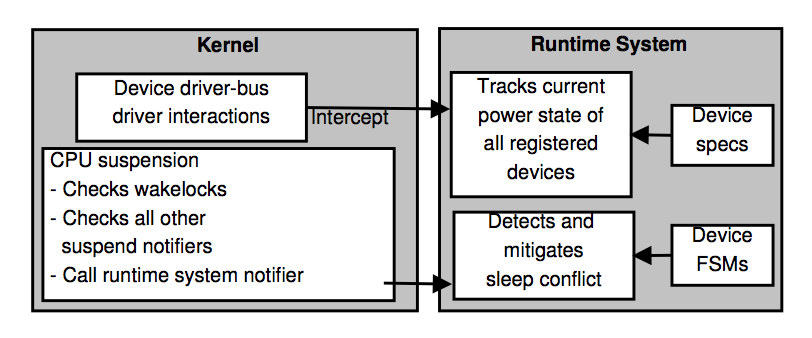
\includegraphics{hypnos-arquitecture.png}
}

\frame{
    \frametitle{Chequeo de condiciones}
    En algún punto cuando el SOC/CPU esta a punto de entrar en estado de suspencion se checkea:

    \begin{itemize}
        \item Si todos los dispositivos estan ya en estado de suspension
        \item Si algunos no, entonces trata de determinar si los drivers invocaron algun mecanismo que asegure que el sistema vaya a estar despierto transcurrido el periodo de tiempo en el cual la transicion del estado de energia vaya a ser llevada a cabo.
    \end{itemize}
    
}

\frame{
    \frametitle{Evitar Conflictos Online}
    Cuando el suspend notifier de HYPNOS es invocado al final del proceso de suspensión del sistema se checkean  las condiciones  necesarias para que ocurra un sleep conflict y se ejecutan los algoritmos necesarios para evitarlo.
}


\begin{frame}[fragile]
    \frametitle{Pseudocódigo (1)}
    \begin{alltt}
    	\textbf{for} all devices \textbf{not in} base state \textbf{do}
            \textbf{if} next transition is end of utilization \textbf{then}
                return \textbf{false}
            \textbf{end} \textbf{if}
            ...
        \textbf{end for}
        return \textbf{true}
    \end{alltt}
\end{frame}

\begin{frame}[fragile]
    \frametitle{Pseudocódigo (2)}
    \begin{alltt}
    	\textbf{for} all devices \textbf{not in} base state \textbf{do}
            ...
            \textbf{if} next transition \textbf{is} timeout \textbf{then}
                next wakeup time = rtc get alarm(..)
                \textbf{if} next wakeup time > timeout time \textbf{then}
                    rtc set alarm( timeout time );
                \textbf{end} \textbf{if}
            \textbf{end} \textbf{if}
            ...
        \textbf{end for}
        return \textbf{true}
    \end{alltt}
\end{frame}

\begin{frame}[fragile]
    \frametitle{Pseudocódigo (3)}
    \begin{alltt}
    	\textbf{for} all devices \textbf{not in} base state \textbf{do}
           ...
            \textbf{if} next transition \textbf{is} external event \textbf{then}
            	\textbf{if} device has not registered hardware wakeup \textbf{then}
                	return \textbf{false}
            	\textbf{end} \textbf{if}
            \textbf{end} \textbf{if}
            ...
        \textbf{end for}
        return \textbf{true}
    \end{alltt}
\end{frame}

\begin{frame}[fragile]
    \frametitle{Pseudocódigo (4)}
    \begin{alltt}
    	\textbf{for} all devices \textbf{not in} base state \textbf{do}
            ...
            \textbf{if} next transition \textbf{is} user input \textbf{then}
                return \textbf{false}
            \textbf{end} \textbf{if}
        \textbf{end for}
        return \textbf{true}
    \end{alltt}
\end{frame}

\frame{
    \frametitle{Wakelock de inactividad}
    Recordemos que cuando el sistema esta prendido, el CPU usa el RTC timer para reintentar suspenderse cada 20ms. La politica de suspensión por inactividad, que suspende el sistema luego de 15 segundos de inactividad del usuario es implementada por el manager de energía del kernel  que retiene un wakelock especial para este propósito por ese período. 
}

\frame{
    \frametitle{Testeo preliminar}
    Cuando un driver realiza la transición de su dispositivo a un estado de consumo de energía activo, entonces o se ha invocado un mecanismo de prevención de sleep conflict o no. Si no, tenemos un potencial sleep conflict, pues el sistema podría suspenderse en cualquier momento. Esta condición puede ser verificada forzando al sistema a tratar de ejecutar el proceso de suspención inmediátamente después de que el dispositivo haya entrado en estado de consumo activo de energía. Se logra liberando el wakelock de inactividad
}

\end{document}